\documentclass[final]{article}

% if you need to pass options to natbib, use, e.g.:
%     \PassOptionsToPackage{numbers, compress}{natbib}
% before loading neurips_2019

% ready for submission
% \usepackage{neurips_2019}

% to compile a preprint version, e.g., for submission to arXiv, add add the
% [preprint] option:
%     \usepackage[preprint]{neurips_2019}

% to compile a camera-ready version, add the [final] option, e.g.:
     \usepackage{neurips_2019}

% to avoid loading the natbib package, add option nonatbib:
%     \usepackage[nonatbib]{neurips_2019}

\usepackage[utf8]{inputenc} % allow utf-8 input
\usepackage[T1]{fontenc}    % use 8-bit T1 fonts
\usepackage{hyperref}       % hyperlinks
\usepackage{url}            % simple URL typesetting
\usepackage{booktabs}       % professional-quality tables
\usepackage{amsfonts}       % blackboard math symbols
\usepackage{nicefrac}       % compact symbols for 1/2, etc.
\usepackage{microtype}      % microtypography
\usepackage{graphicx}

\title{Estimating the long-term effect of\\ early treatment initiation in Parkinson's disease\\using observational data}

% The \author macro works with any number of authors. There are two commands
% used to separate the names and addresses of multiple authors: \And and \AND.
%
% Using \And between authors leaves it to LaTeX to determine where to break the
% lines. Using \AND forces a line break at that point. So, if LaTeX puts 3 of 4
% authors names on the first line, and the last on the second line, try using
% \AND instead of \And before the third author name.

\author{%
  Lieneke van den Heuvel\\
  Donders Institute\\
  Department of Neurology\\
  Radboud university medical centre\\
  \And
  Luc J.W. Evers\\
  Donders Institute\\
  Department of Neurology\\
  Radboud university medical centre\\
  \And
  Marjan J. Meinders\\
  Radboud Institute for Health Sciences\\
  Radboud university medical centre\\
  \And
  Bart Post\\
   Donders Institute\\
  Department of Neurology\\
  Radboud university medical centre\\
  \And 
  Anne M. Stiggelbout\\
  Medical Decision Making\\
  Department of Biomedical Data Sciences\\
  Leiden University Medical Centre\\
  \And
  Tom Heskes\\
   Institute for Computing and Information Sciences\\
   Radboud University\\
  \And
   Bastiaan R. Bloem\\
      Donders Institute\\
  Department of Neurology\\
  Radboud university medical centre\\
   \And
   Jesse H. Krijthe\\
   Institute for Computing and Information Sciences\\
   Radboud University\\
  % examples of more authors
  % \And
  % Coauthor \\
  % Affiliation \\
  % Address \\
  % \texttt{email} \\
  % \AND
  % Coauthor \\
  % Affiliation \\
  % Address \\
  % \texttt{email} \\
  % \And
  % Coauthor \\
  % Affiliation \\
  % Address \\
  % \texttt{email} \\
  % \And
  % Coauthor \\
  % Affiliation \\
  % Address \\
  % \texttt{email} \\
}

\begin{document}

\maketitle

%Parkinson’s disease (PD) is a neurodegenerative disorder, characterized by the loss of dopaminergic neurons within the substantia nigra region of the brain. While dopamine replacement therapy is effectively applied to treat symptoms of PD in the large majority of patients, patients and physicians may choose to delay initiation of dopamine replacement therapy for concerns of toxicity or development of side-effects. Although randomized controlled trials (RCTs) have evaluated the effect of early versus late start of treatment, the influence of dopaminergic treatment on the long-term disease progression is still not fully clear. The goal of this work is to find out what evidence longitudinal observational data can bring to bear on the question of early or delayed medication treatment initiation in Parkinson's disease, by estimating the long-term causal effect of the duration of PD medication treatment during the first two years of follow-up on clinical outcomes of interest, using methods that adjust for time-varying confounding. Aside from estimates for these effects themselves, the analysis also shows the importance of complex causal models to take time-varying confounding into account when answering questions such as these.

%\begin{abstract}
%  The abstract paragraph should be indented \nicefrac{1}{2}~inch (3~picas) on
%  both the left- and right-hand margins. Use 10~point type, with a vertical
%  spacing (leading) of 11~points.  The word \textbf{Abstract} must be centered,
%  bold, and in point size 12. Two line spaces precede the abstract. The abstract
%  must be limited to one paragraph.
%\end{abstract}

\section*{Background}
Parkinson's disease (PD) is a neurodegenerative disorder, characterized by the loss of dopaminergic neurons within the substantia nigra region of the brain. The main symptomatic treatments in PD focus on dopamine replacement. Both patients and physicians may choose, however, to delay initiation of dopamine replacement therapy in Parkinson's disease for various reasons, including concerns regarding the toxicity of therapy and early development of treatment-related side effects, such as dyskinesias and motor fluctuations. 

Although randomized controlled trials (RCTs) have evaluated the effect of early versus late start of treatment [3,4], the influence of dopaminergic treatment on the long-term disease progression is still not fully clear [1,2]. Additionally, RCTs come with some limitations including relatively short follow-up and having non-representative study samples. As such, RCTs usually do not account for the typical heterogeneity within a real-life population. Observational data, with less strict in- and exclusion criteria and self-selection, may be more representative of the true patient population, and (increasingly) more readily available, but offer their own challenges in terms of statistical modelling and interpretation of results. We have two main goals with this work: 1. Find out what evidence longitudinal observational data can bring to bear on the question of early medication treatment initiation in Parkinson's disease, by estimating the long-term effect of the duration of PD medication treatment in the first two years of follow-up on clinical outcomes of interest. 2. Show that causal inference methods that take time-varying confounding into account are essential when estimating such effects.

\section*{Data \& Outcomes}
The Parkinson Progression Markers Initiative (PPMI) [5] is a multi-centre longitudinal observational study with long follow-up of up to 8 years. We used the PPMI cohort with $423$ de novo PD patients to estimate the treatment effect of a year of PD medication therapy during the first two years of follow-up on outcomes in years 2, 3 and 4. Our primary outcome of interest is the total MDS-UPRS part III (off) score, an examination of movement-related symptoms. Secondary outcomes included the MDS-UPDRS part I (nonmotor experiences of daily living) and II (motor experiences of daily living), the Montreal Cognitive Assessment, Schwab and England Activities of Daily Living scale and the presence of dyskinesias and motor fluctuations. For the analyses presented here, we used information on $302$ patients who started using PD medication within two years since the start of the study. Additionally, we are also interested in estimating the effect of Levodopa therapy specifically (instead of all PD medication combined), while recognizing that the group of patients that used Levodopa exclusively is small ($n=82$).

\section*{Methods}
\begin{figure}
  \centering
  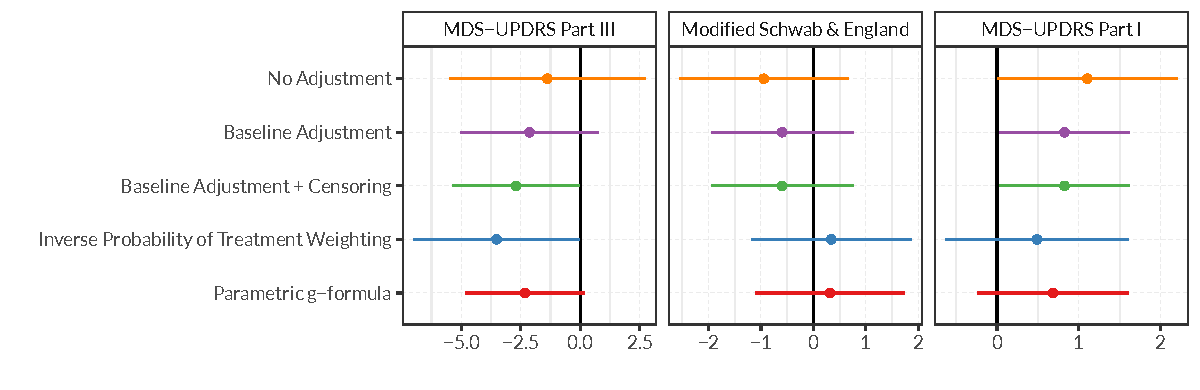
\includegraphics[width=\textwidth]{different-models.pdf}
  \caption{Effect of an additional year of PD medication therapy on outcomes after two years estimated using different methods. Intervals indicate $\pm 2$ times the standard deviation of the estimator, estimated using $1000$ bootstrap replicates. For Modified Schwab \& England, higher scores correspond to improved disease outcomes, while for MDS-UPDRS part I and III, lower scores correspond to more beneficial outcomes. Note that adjusting for more of the confounding effects shifts the estimates to more beneficial outcomes for all three measures, indicating the importance of using these types of methods when analyzing this data.}
  \label{fig1}
\end{figure}
The challenge we try to address in this work is to adjust for (time-varying) confounding introduced by the patient's disease state influencing the treatment initiation decision and vice versa. To do this, we use Marginal Structural Models using Inverse Probability Weighting and the parametric g-formula [6]. Agreement between these two methods will increase credence that the results are not merely the effect of one of the models being mis-specified.

For inverse probability of treatment weighting [7], we fit models for treatment assignment (start therapy vs. no start of therapy among patients who have not started yet) at each visit. The models used are logistic regression models that predict therapy initiation in the period following a planned visit, based on MDS-UPDRS I, II and III scores, Modified Schwab-England scores, MoCA, age, sex, years of education and disease duration. We use these models to weight the observations in a marginal structural model where we estimate the effect of treatment duration on the outcomes. To adjust for the censoring of patients by loss of follow-up, we also use inverse probability weights for the probability of censoring, using models that have the same structure (but different parameter estimates) as those for the treatment assignment.

For the parametric g-formula, we need to construct disease progression models for the confounders and outcomes at each visit, based on data from the previous visits and the treatment status. We use linear regression models at each step, using as covariates MDS-UPDRS subscores, MoCA, Modified Schwab-England scores, Age, Sex, Years of Education and disease duration. Using these models, for each patient starting with their baseline measurements, we simulate 100 patient disease trajectories for each treatment policy of interest: starting therapy at year 0, 0.5, 1 or 1.5. We then estimate the linear effect of an additional year of treatment using a marginal structural model, as in the case of inverse probability of treatment weighting.

For comparison, we also fit a model that does not take confounding into account, directly comparing groups of patients that had different lengths of medication therapy during the first two years after the start of the study. We also extend this naive model to a linear model that adjusts for the value of the outcome at baseline. We further extend this second model by using inverse probability weighting to correct only for censoring, as described above.

\section*{Results}
Figure~\ref{fig1} shows that the models that take the time-varying nature of the treatment initiation into account move the estimates in the direction of more beneficial outcomes for all three outcomes. This is what one would expect when adjusting for (time-varying) confounding in this situation, since the simpler models may attribute observing bad outcomes to the intervention itself, rather than the bad disease state that caused the early intervention.

Estimates of our main causal quantity of interest (the effect of one additional year of therapy on MDS-UPDRS III outcomes at year 2, 3 and 4) are shown in Figure~\ref{fig2}. Based on these estimates, early initiation of PD medication treatment does not lead to higher/worse MDS-UPDRS III scores in the first four years of the disease, as is sometimes feared. There is even an indication that early initiation lowers scores, corresponding to beneficial effects, for which we offer multiple explanations. We found no significantly different treatment effect for early versus delayed start of PD medication for the side effects we considered, in part because the uncertainty for these estimators is very large (not shown). 


\begin{figure}
  \centering
  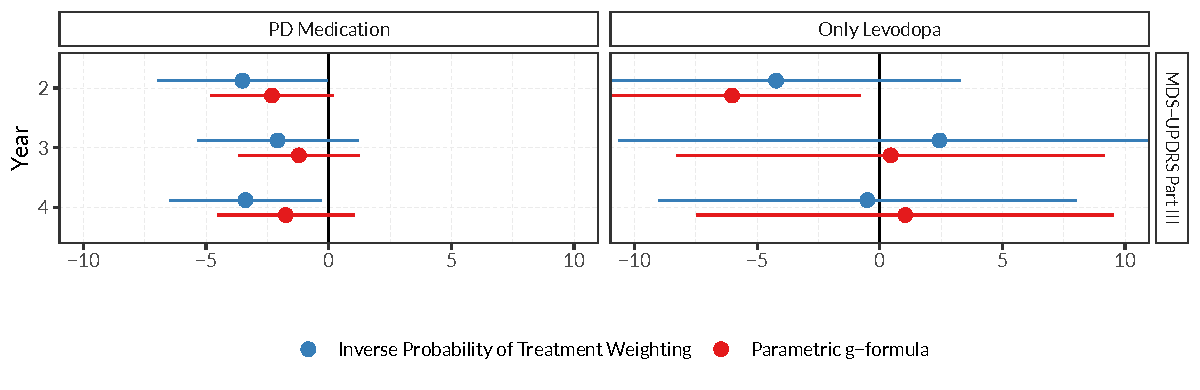
\includegraphics[width=\textwidth]{main-outcomes.pdf}
  \caption{Effect of one year of PD medication respectively Levodopa treatment during the first two years of follow-up. Effect on MDS-UPDRS part III subscore measured at year 2, 3 and 4, for inverse probability of treatment weighting and the parametric g-formula. Lower scores correspond to better disease outcomes. Intervals indicate $\pm 2$ times the standard deviation of the estimator, estimated using $1000$ bootstrap replicates.}
  \label{fig2}
\end{figure}

\section*{Discussion}
There are several important properties of the data and the analysis that have to be taken into account when interpreting these results. The main outcome, for instance, may be affected by so-called long duration response of medication: while the research protocol tries to make sure direct symptomatic effects of the medication are reduced by making sure patients did not take medication in the last 12 hours before doing the examination, this time period is likely not long enough to wash out all direct symptomatic effects. We try to reduce this effect by only considering patients who are using medication at the time of the measurement. 

Additionally, the assumptions of (sequential) consistency, exchangeability, positivity and correct model specification needed for the causal models need to be taken in mind when assessing the claims of the causal effect estimates. Aside from these conceptual challenges, real-world observational data poses practical challenges as well: even with a large and well-run study such as PPMI, unexpected missing data and other inconsistencies require choices and assumptions that may affect the results.

\section*{Conclusions}
We find no evidence for differential effects of early or delayed start of Parkinson medication therapy for most outcomes and tentative positive effects for some of the main outcomes considered here. The former is in line with earlier findings from clinical trials, while the latter offers potentially interesting new evidence in favour of initiating PD medication therapy early. Our analysis further shows that taking time-varying confounding into account is essential in drawing correct conclusions when studying questions such as ours. 
While applying causal models to observational studies has several advantages over clinical trials, their results have to be interpreted in the context of the assumptions underlying these methods. When taking these limitations into account, these analyses can offer an additional source of evidence for the effect of early treatment initiation in de novo Parkinson's patients. With the increasing availability of large observational cohort studies, these type of analyses can offer a valuable complement to the highly useful, but hard to obtain results from randomized controlled trials.

\subsubsection*{Acknowledgments}
This project is funded by ZonMw project 91215076 “Big Data for Personalised Medicine.” We gratefully acknowledge the PPMI for use of the data.

\section*{References}

[1] Olanow, C.W., Levodopa: effect on cell death and the natural history of Parkinson's disease. Mov Disord, 2015. 30(1): p. 37-44.

[2] Parkkinen, L., et al., Does levodopa accelerate the pathologic process in Parkinson disease brain? Neurology, 2011. 77(15): p. 1420-6.

[3] Fahn, S., et al., Levodopa and the progression of Parkinson's disease. N Engl J Med, 2004. 351(24): p. 2498-508.

[4] Verschuur, C.V.M., et al., Randomized Delayed-Start Trial of Levodopa in Parkinson's Disease. N Engl J Med, 2019. 380(4): p. 315-324.

[5] Parkinson Progression Marker Initiative, The Parkinson Progression Marker Initiative (PPMI). Prog Neurobiol, 2011. 95(4): p. 629-35.

[6] Hernan, M.A. and J.M. Robins, Causal Inference. Boca Raton: Chapman \& Hall/CRC. 2019.

[7] Robins, J.M., M.A. Hernan, and B. Brumback, Marginal structural models and causal inference in epidemiology. Epidemiology, 2000. 11(5): p. 550-60

\end{document}
